\documentclass{standalone}
\usepackage{tikz}
\usepackage{amsmath}
\usepackage{amssymb}
\usepackage{mathrsfs}

\begin{document}

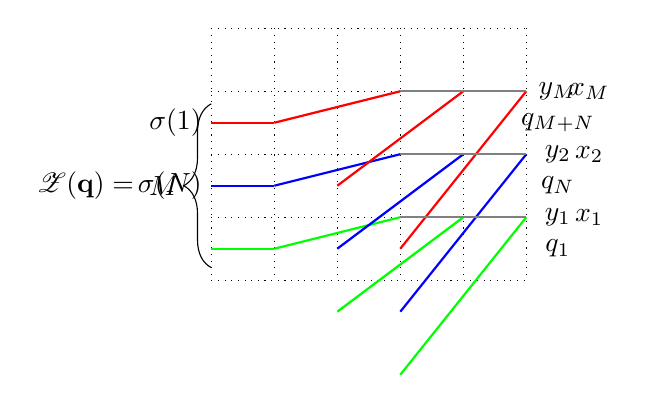
\begin{tikzpicture}[scale=0.8]

% Draw the main structure
\foreach \x in {0,1,2,3,4} {
    \draw[dotted] (0,-\x) -- (5,-\x);
}

\foreach \y in {0,1,2,3,4,5} {
    \draw[dotted] (\y,0) -- (\y,-4);
}

% Horizontal lines with colors
\draw[thick, red] (0,-1.5) -- (1,-1.5);
\draw[thick, blue] (0,-2.5) -- (1,-2.5);
\draw[thick, green] (0,-3.5) -- (1,-3.5);

% Diagonal lines crossing
\foreach \x/\y in {1/-1.5, 2/-2.5, 3/-3.5} {
    \draw[thick, red] (\x,\y) -- (\x+2,-1);
    \draw[thick, blue] (\x,\y-1) -- (\x+2,-2);
    \draw[thick, green] (\x,\y-2) -- (\x+2,-3);
}

% Horizontal lines on the right
\draw[thick, gray] (3,-1) -- (5,-1);
\draw[thick, gray] (3,-2) -- (5,-2);
\draw[thick, gray] (3,-3) -- (5,-3);

% Right side labels
\node at (5.5,-1) {$y_M$};
\node at (5.5,-2) {$y_2$};
\node at (5.5,-3) {$y_1$};

\node at (5.5,-1.5) {$q_{M+N}$};
\node at (5.5,-2.5) {$q_N$};
\node at (5.5,-3.5) {$q_1$};

\node at (6,-1) {$x_M$};
\node at (6,-2) {$x_2$};
\node at (6,-3) {$x_1$};

% Left side labels
\node[left] at (0,-1.5) {$\sigma(1)$};
\node[left] at (0,-2.5) {$\sigma(N)$};

% Brackets
\draw[decorate,decoration={brace,amplitude=10pt}] (0,-3.8) -- (0,-1.2) node [midway,xshift=-0.6cm] {$M$};

% Z(q) label
\node at (-2,-2.5) {$\mathscr{Z}(\mathbf{q}) = $};

\end{tikzpicture}

\end{document}